\documentclass[10pt]{article}

\addtolength{\oddsidemargin}{-.875in}
\addtolength{\evensidemargin}{-.875in}
\addtolength{\textwidth}{1.75in}

\usepackage{graphicx}
\usepackage[usenames,dvipsnames]{xcolor, colortbl} %used for font color
\usepackage{amssymb} %maths
\usepackage{amsmath} %maths
\usepackage{pifont}
\usepackage{framed}
\usepackage[utf8]{inputenc} %useful to type directly diacritic characters
\newcommand{\cmark}{\ding{51}}%
\definecolor{mygray}{rgb}{0.85,0.85,0.85}
\newcommand{\bs}{\boldsymbol}

\pagestyle{empty}
\begin{document}

\begin{framed}

\begin{center}
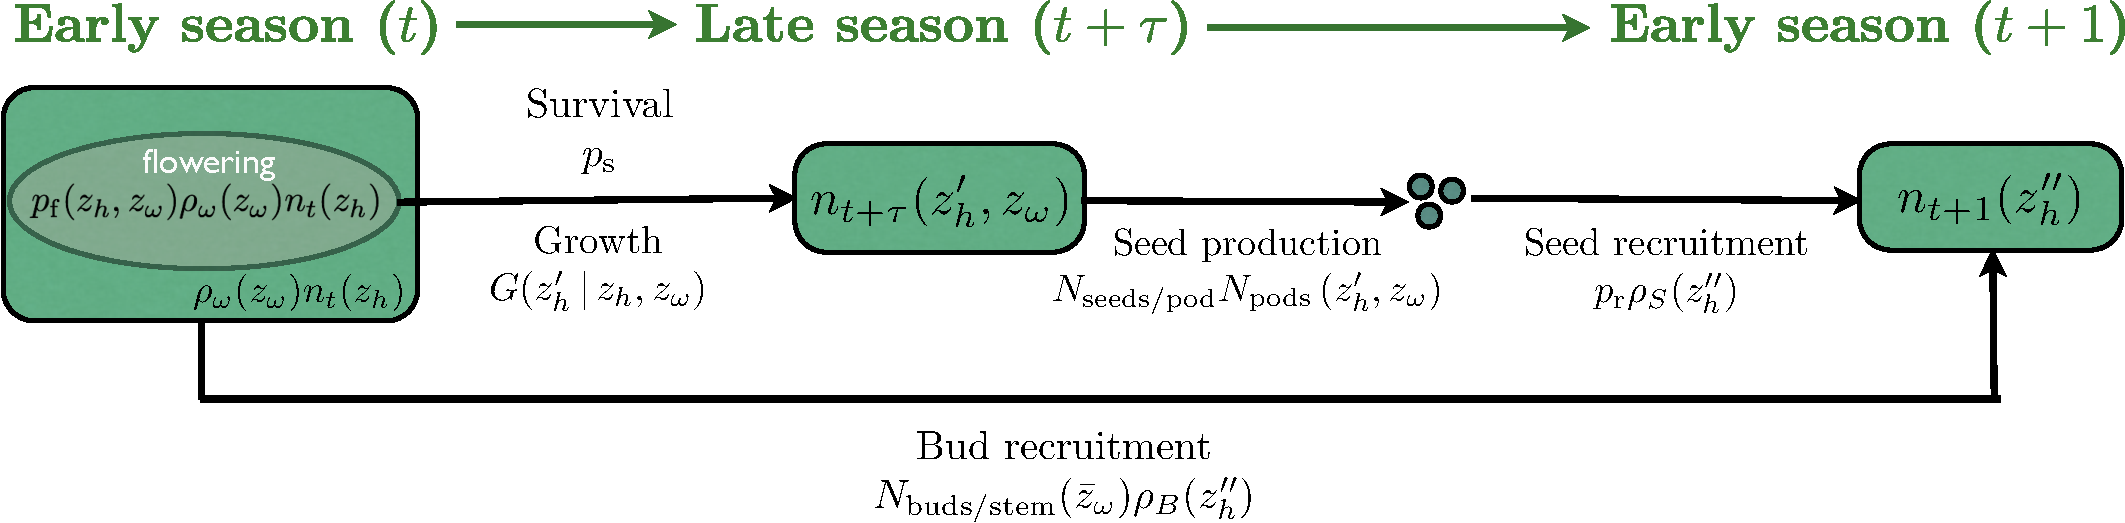
\includegraphics[width=5.5in]{LifeCycleDiagram.pdf}

\begin{align*}
n_{t+1}(z_{h}^{\prime\prime}) = \ & \underbrace{\rho_{B}(z_{h}^{\prime\prime})N_{\mathrm{buds/stem}}(\bar{z}_{\omega})\int\int \rho_{\omega}(z_{\omega})n_{t}(z_{h})\, dz_{h}dz_{\omega}}_\text{Clonal pathway} \ + \\
  & \underbrace{p_{\mathrm{r}}\rho_{S}(z_{h}^{\prime\prime})N_{\mathrm{seeds/pod}}\int\int N_{\mathrm{pods}}\left(z_{h}^{\prime},z_{\omega}\right)n_{t+\tau}(z_{h}^{\prime},z_{\omega}) \,dz_{h}^{\prime}dz_{\omega}}_\text{Sexual pathway} \\
n_{t+\tau}(z_{h}^{\prime},z_{\omega}) = \ & \int p_{\mathrm{s}} G(z_{h}^{\prime}\, | \, z_{h},z_{\omega})p_{\mathrm{f}}(z_{h},z_{\omega})\rho_{\omega}(z_{\omega})n_{t}(z_{h})\, dz_{h}
\end{align*}

\end{center}

\vspace{0.35in}

\centering
\begin{tabular}{ |l|l|c| }
\hline
\rowcolor{mygray} 
Terms & Description & Functional form \\ \hline
$p_{\mathrm{s}}$ & Probability of ramet survival & $logit^{-1}(\alpha + u_{\alpha\cdot} + u_{z_{\omega}\cdot})$ \\
$G(z_{h}^{\prime}\, | \, z_{h},z_{\omega})$ & Growth & $\begin{array}{ll}\alpha \ + & \!\!\!\beta_{z_{h}} + \beta_{z_{\omega}} + \beta_{z_{h}:z_{\omega}} + \\ & \!\!\!u_{\alpha\cdot} + u_{z_{h}\cdot} + u_{z_{\omega}\cdot} + N(0,\sigma^2)\end{array}$ \\
$p_{\mathrm{f}}(z_{h},z_{\omega})$ & Probability of flowering & $logit^{-1}(\alpha + \beta_{z_{h}} + \beta_{z_{\omega}} + \beta_{z_{h}:z_{\omega}} + u_{\alpha\cdot})$ \\ 
$N_{\mathrm{pods}}\left(z_{h}^{\prime},z_{\omega}\right)$ & Number of pods & $exp(\alpha + \beta_{z_{h}} + \beta_{z_{\omega}} + u_{\alpha\cdot} + u_{z_{h}\cdot} + u_{z_{\omega}\cdot})$ \\ 
$N_{\mathrm{seeds/pod}}$ & Number of seeds per pod & $\alpha$ \\
$N_{\mathrm{buds/stem}}(\bar{z}_{\omega})$ & Number of buds per stem & $exp(\alpha + \beta_{\bar{z}_{\omega}})$ \\ 
$p_{\mathrm{r}}$ & Probability of seed recruitment & $\alpha$ \\
$\rho_{\omega}(z_{\omega})$ & Herbivory distribution & $\left\{\begin{array}{ll}1-p_{\omega}, & z_{\omega} = 0, \\ p_{\omega}\ln N(\mu, \sigma^2)^{*}, & z_{\omega} > 0\end{array}\right.$ \\
$\rho_{S}(z_{h}^{\prime\prime})$ & Seed recruit distribution & $\ln N(\mu, \sigma^2)^{*}$ \\
$\rho_{B}(z_{h}^{\prime\prime})$ & Bud recruit distribution & $N(\mu, \sigma^2)$ \\
\hline
\end{tabular}

\end{framed}

\end{document}